\documentclass[tikz,border=2pt]{standalone}
\usepackage{amsmath}
\usepackage{pgfplots}
\pgfplotsset{compat=1.18}
\usetikzlibrary{arrows.meta}
\begin{document}
% Farkas' lemma, Example 1: K = Cone({A1,A2}) with A1=(1,0), A2=(1,1).
% (a) b=(2,1)=A1+A2 lies in K, x=(1,1). (b) b=(0,2) lies outside K; nearest point q=(1,1), y=q-b=(1,-1),
% hyperplane H: x1=x2 through 0 has K on the side y^T x >= 0 and b on the side y^T x < 0.
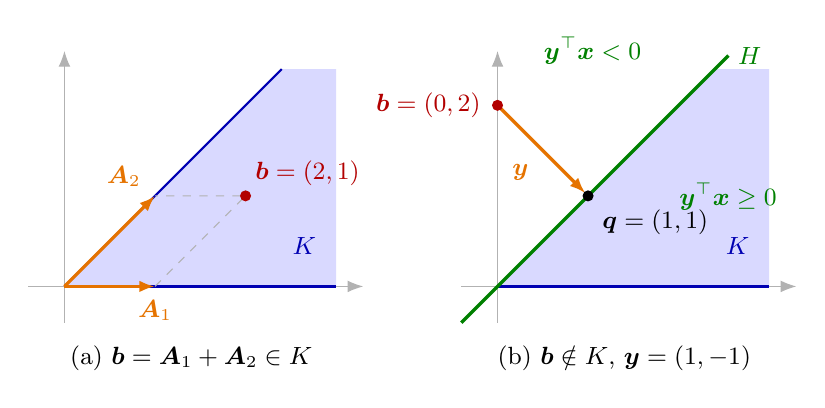
\begin{tikzpicture}[font=\small, >={Latex[length=2mm]}, x=1.15cm, y=1.15cm]
  % ---------------- (a) b in K ----------------
  \begin{scope}
    \fill[blue!15] (0,0) -- (3,0) -- (3,2.4) -- (2.4,2.4) -- cycle;
    \draw[gray!60, ->] (-0.4,0) -- (3.3,0);
    \draw[gray!60, ->] (0,-0.4) -- (0,2.6);
    \draw[blue!70!black, thick] (0,0) -- (3,0);
    \draw[blue!70!black, thick] (0,0) -- (2.4,2.4);
    \node[blue!70!black] at (2.65,0.45) {$K$};
    \draw[gray!60, dashed] (1,0) -- (2,1) -- (1,1);
    \draw[orange!90!black, very thick, ->] (0,0) -- (1,0);
    \draw[orange!90!black, very thick, ->] (0,0) -- (1,1);
    \node[orange!90!black, anchor=north] at (1,-0.05) {$\boldsymbol{A}_1$};
    \node[orange!90!black, anchor=south east] at (0.95,1.0) {$\boldsymbol{A}_2$};
    \fill[red!70!black] (2,1) circle (2pt);
    \node[red!70!black, anchor=south west] at (2.0,1.0) {$\boldsymbol{b}=(2,1)$};
    \node[anchor=north] at (1.4,-0.55) {(a) $\boldsymbol{b}=\boldsymbol{A}_1+\boldsymbol{A}_2\in K$};
  \end{scope}
  % ---------------- (b) b not in K ----------------
  \begin{scope}[xshift=5.5cm]
    \fill[blue!15] (0,0) -- (3,0) -- (3,2.4) -- (2.4,2.4) -- cycle;
    \draw[gray!60, ->] (-0.4,0) -- (3.3,0);
    \draw[gray!60, ->] (0,-0.4) -- (0,2.6);
    \draw[blue!70!black, thick] (0,0) -- (3,0);
    \node[blue!70!black] at (2.65,0.45) {$K$};
    % separating hyperplane H: x1 = x2
    \draw[green!50!black, very thick] (-0.4,-0.4) -- (2.55,2.55);
    \node[green!50!black, anchor=west] at (2.55,2.55) {$H$};
    \node[green!50!black, anchor=north west] at (1.9,1.25) {$\boldsymbol{y}^{\top}\boldsymbol{x}\geq0$};
    \node[green!50!black, anchor=south] at (1.05,2.35) {$\boldsymbol{y}^{\top}\boldsymbol{x}<0$};
    % b, q and y = q - b
    \draw[orange!90!black, very thick, ->] (0,2) -- (0.97,1.03);
    \node[orange!90!black, anchor=north east] at (0.45,1.45) {$\boldsymbol{y}$};
    \fill (1,1) circle (2pt);
    \node[anchor=north west] at (1.05,0.95) {$\boldsymbol{q}=(1,1)$};
    \fill[red!70!black] (0,2) circle (2pt);
    \node[red!70!black, anchor=east] at (-0.08,2) {$\boldsymbol{b}=(0,2)$};
    \node[anchor=north] at (1.4,-0.55) {(b) $\boldsymbol{b}\notin K$, $\boldsymbol{y}=(1,-1)$};
  \end{scope}
\end{tikzpicture}
\end{document}
